\documentclass[11pt,a4paper]{article}
\usepackage{../common/polycopie_style}

\begin{document}

\makepolycopieheader{Corrélation, Régression Linéaire \& Gammes d'Étalonnage}{Modélisation Statistique, Moindres Carrés Ordinaires \& Inférence Analytique}{CHAPITRE 3}

\section{Introduction : La Transduction du Signal Analytique}

En biochimie et biologie médicale, les automates de laboratoire ne comptent jamais directement le nombre de molécules dans une éprouvette :
\begin{itemize}[leftmargin=*, label=\faAngleRight]
  \item Le \textbf{spectrophotomètre} mesure l'atténuation d'un faisceau lumineux ($A_{595}$ dans un dosage de Bradford).
  \item Le \textbf{luminomètre ELISA} mesure une intensité de fluorescence émise par une sonde enzymatique (RLU).
  \item Le \textbf{thermocycleur qPCR} quantifie un cycle seuil d'amplification ($C_t$).
\end{itemize}

Pour convertir ce signal physique abstrait $Y$ en concentration massique ou molaire réelle $X$ ($\mu\text{g/mL}$, $\text{mM}$), l'expérimentateur prépare une \textbf{gamme étalon} de concentrations connues, mesure les signaux correspondants, et ajuste un modèle mathématique.

\begin{conceptbox}{Corrélation vs Régression : Une Différence Fondamentale}
\begin{itemize}[leftmargin=*, label=\faCheck]
  \item \textbf{La Corrélation ($r$) :} Mesure la force et le sens de l'association linéaire \textbf{symétrique} entre deux variables aléatoires conjointes ($X$ et $Y$). Aucune variable n'explique l'autre (ex : corrélation entre les transaminases ASAT et ALAT lors d'une cytolyse hépatique).
  \item \textbf{La Régression ($Y = f(X) + \varepsilon$) :} Établit une relation fonctionnelle \textbf{directionnelle et causale}. La variable indépendante $X$ (fixée sans erreur par le manipulateur) prédit la variable dépendante $Y$ (réponse expérimentale bruitée).
\end{itemize}
\end{conceptbox}

\section{Le Coefficient de Corrélation Linéaire de Pearson ($r$)}

Pour deux variables quantitatives continues $X$ et $Y$ mesurées sur $n$ individus, le coefficient de Pearson mesure l'alignement des points :
\begin{equation*}
  r = \frac{\sum_{i=1}^n (x_i - \bar{x})(y_i - \bar{y})}{\sqrt{\sum_{i=1}^n (x_i - \bar{x})^2} \cdot \sqrt{\sum_{i=1}^n (y_i - \bar{y})^2}} = \frac{SP_{xy}}{\sqrt{SS_{xx} \cdot SS_{yy}}}
\end{equation*}
avec $-1 \le r \le +1$.

\begin{warnbox}{Corrélation n'est pas Causalité}
Deux biomarqueurs peuvent présenter une corrélation de $r = 0.98$ sous l'effet d'une troisième variable cachée (variable confondante, ex : la masse corporelle ou la sévérité globale de la pathologie), sans qu'aucun ne cause directement l'autre.
\end{warnbox}

\section{Le Modèle Linéaire Simple \& Moindres Carrés Ordinaires (MCO)}

Le modèle statistique postule :
\begin{equation*}
  y_i = \beta_0 + \beta_1 x_i + \varepsilon_i \quad \text{avec } \varepsilon_i \sim \mathcal{N}(0, \sigma^2)
\end{equation*}

La droite des moindres carrés $\hat{y}_i = a x_i + b$ minimise la somme des carrés des écarts verticaux $\sum (y_i - \hat{y}_i)^2$ :
\begin{align*}
  a &= \frac{SP_{xy}}{SS_{xx}} = \frac{\sum (x_i - \bar{x})(y_i - \bar{y})}{\sum (x_i - \bar{x})^2} \quad \text{(Pente = Sensibilité analytique)} \\[1mm]
  b &= \bar{y} - a \bar{x} \quad \text{(Ordonnée à l'origine = Signal du blanc réactif)}
\end{align*}

\begin{biobox}{Interprétation Biochimique des Paramètres}
\begin{itemize}[leftmargin=*, label=\faAngleRight]
  \item \textbf{Pente $a$ (Sensibilité) :} Variation d'absorbance par unité de concentration ($\Delta A / \Delta C$). Plus $a$ est élevée, plus la méthode détecte de fines variations.
  \item \textbf{Ordonnée $b$ (Bruit de fond) :} Absorbance théorique à concentration nulle ($X = 0$). Un test de Student teste si $b = 0$.
\end{itemize}
\end{biobox}

\section{Qualité de l'Ajustement \& Décomposition de la Variance}

La dispersion totale du signal optique $SCT$ se décompose en :
\begin{equation*}
  \sum (y_i - \bar{y})^2 = \sum (\hat{y}_i - \bar{y})^2 + \sum (y_i - \hat{y}_i)^2 \iff SCT = SCE + SCR
\end{equation*}
\begin{itemize}[leftmargin=*, label=\faCheck]
  \item \textbf{Coefficient de Détermination ($R^2 = r^2$) :} 
  \begin{equation*}
    R^2 = \frac{SCE}{SCT} = 1 - \frac{SCR}{SCT}
  \end{equation*}
  Représente la fraction de variance du signal optique expliquée par la concentration en étalon.
  \item \textbf{Variance Résiduelle ($s_{y/x}^2$) :} 
  \begin{equation*}
    s_{y/x}^2 = \frac{SCR}{n - 2} \implies s_{y/x} = \sqrt{\frac{\sum (y_i - \hat{y}_i)^2}{n - 2}}
  \end{equation*}
\end{itemize}

\section{Prédiction Inverse \& Formule de Mandel (Dosage d'Inconnus)}

Pour un échantillon biologique inconnu donnant une réponse moyenne $y_0$ (moyenne de $m$ lectures répliquées) :
\begin{equation*}
  \hat{x}_0 = \frac{y_0 - b}{a}
\end{equation*}
L'erreur standard sur cette concentration estimée est calculée par la \textbf{formule de Mandel} :
\begin{equation*}
  s_{\hat{x}_0} = \frac{s_{y/x}}{a} \sqrt{\frac{1}{m} + \frac{1}{n} + \frac{(y_0 - \bar{y})^2}{a^2 \cdot SS_{xx}}}
\end{equation*}
L'intervalle de confiance à $95\%$ est :
\begin{equation*}
  IC_{95\%}(\hat{x}_0) = \left[ \hat{x}_0 \pm t_{0.05}(n - 2) \cdot s_{\hat{x}_0} \right]
\end{equation*}

\begin{figurebox}{Gamme d'Étalonnage de Bradford \& Fuseau Hyperbolique de Mandel}
\begin{center}
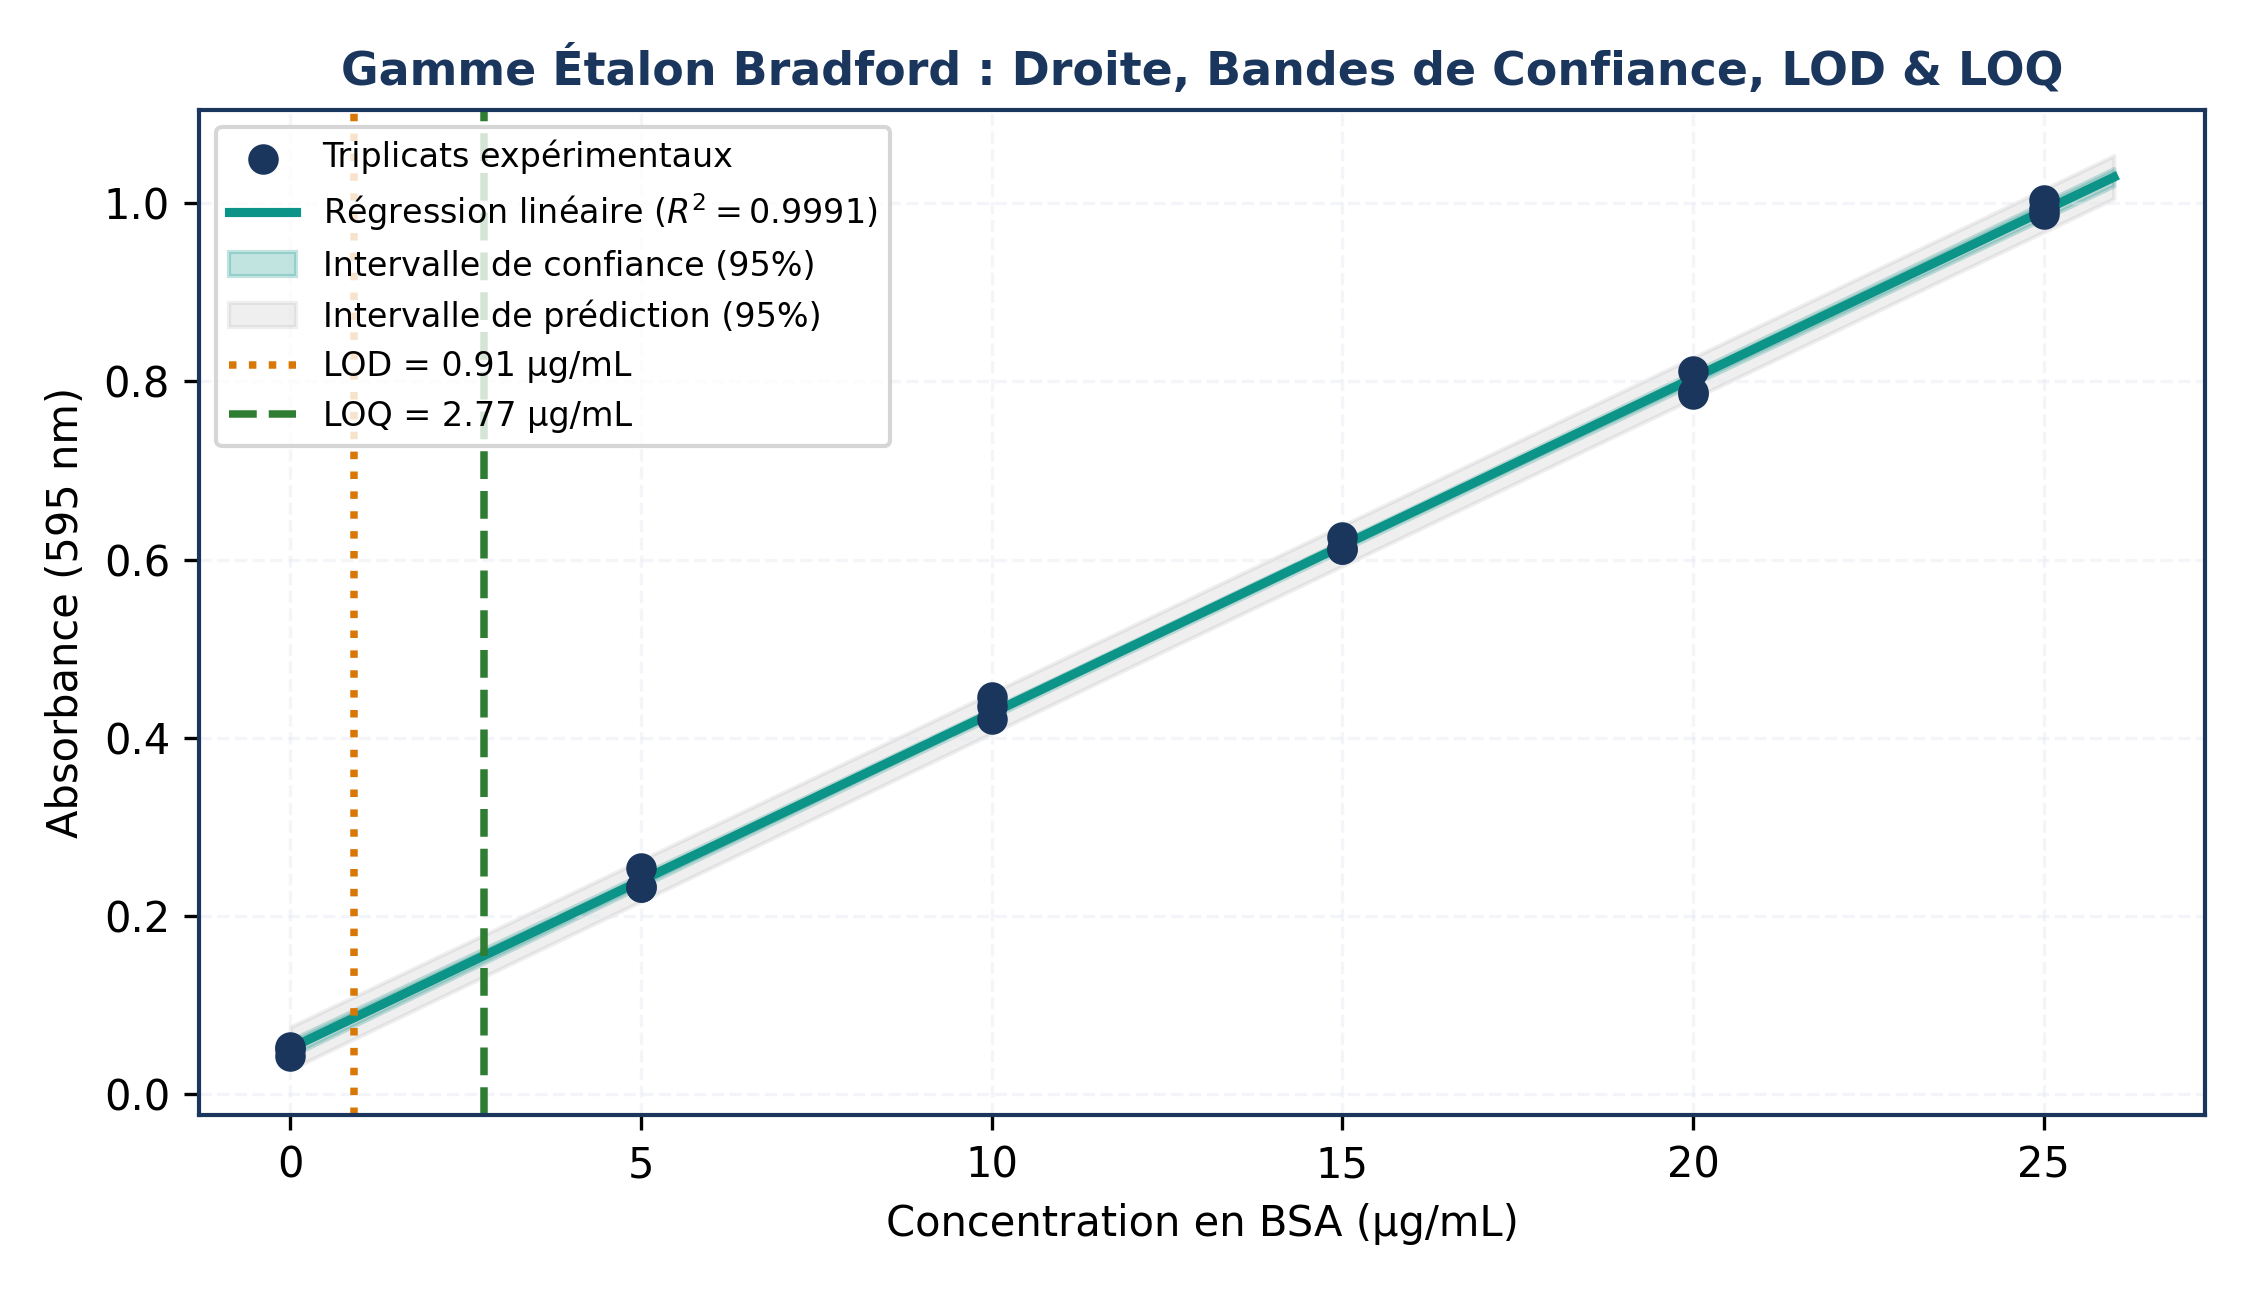
\includegraphics[width=0.84\linewidth]{../../sources/figures/fig03_bradford_calibration.png}
\end{center}
\textbf{Analyse du graphique d'étalonnage spectrophotométrique :}
\begin{itemize}[leftmargin=*, label=\faAngleRight]
  \item \textbf{Droite des Moindres Carrés Ordinaires ($\hat{y} = ax + b$) :} Elle ajuste la relation linéaire théorique entre l'absorbance à $595\,\text{nm}$ et la concentration en protéine standard (BSA). La pente $a$ représente la sensibilité analytique.
  \item \textbf{Bandes de confiance à 95\% (Formule de Mandel) :} Observez le profil caractéristique en sablier (hyperbole) des limites supérieure et inférieure. L'intervalle de confiance est le plus étroit au niveau du barycentre des points $(\bar{x}, \bar{y})$.
  \item \textbf{Conséquence pratique pour l'expérimentateur :} C'est au milieu de la gamme ($[4 - 6]\,\mu\text{g/mL}$) que l'incertitude sur la concentration dosée est minimale. Plus on s'approche des extrémités de la gamme, plus l'incertitude augmente rapidement.
\end{itemize}
\end{figurebox}

\section{Diagnostic des Résidus \& Validation des Hypothèses de Gauss-Markov}

L'estimation par les Moindres Carrés n'est optimale (\textit{théorème de Gauss-Markov : estimateur BLUE}) que si les résidus $\hat{\varepsilon}_i = y_i - \hat{y}_i$ vérifient quatre hypothèses fondamentales :
\begin{enumerate}[leftmargin=*, label=\faCheck\ \textbf{\arabic*.}]
  \item \textbf{Linéarité :} La vraie relation sous-jacente est bien rectiligne ($E(\varepsilon_i) = 0$).
  \item \textbf{Homoscédasticité :} La variance de l'erreur est constante sur toute l'étendue de mesure ($\text{Var}(\varepsilon_i) = \sigma^2$).
  \item \textbf{Normalité :} Les erreurs aléatoires suivent une loi gaussienne $\varepsilon_i \sim \mathcal{N}(0, \sigma^2)$.
  \item \textbf{Indépendance :} Les résidus entre tubes sont mutuellement indépendants ($\text{Cov}(\varepsilon_i, \varepsilon_j) = 0$).
\end{enumerate}

\begin{figurebox}{Les 4 Graphiques Clés du Diagnostic des Résidus}
\begin{center}
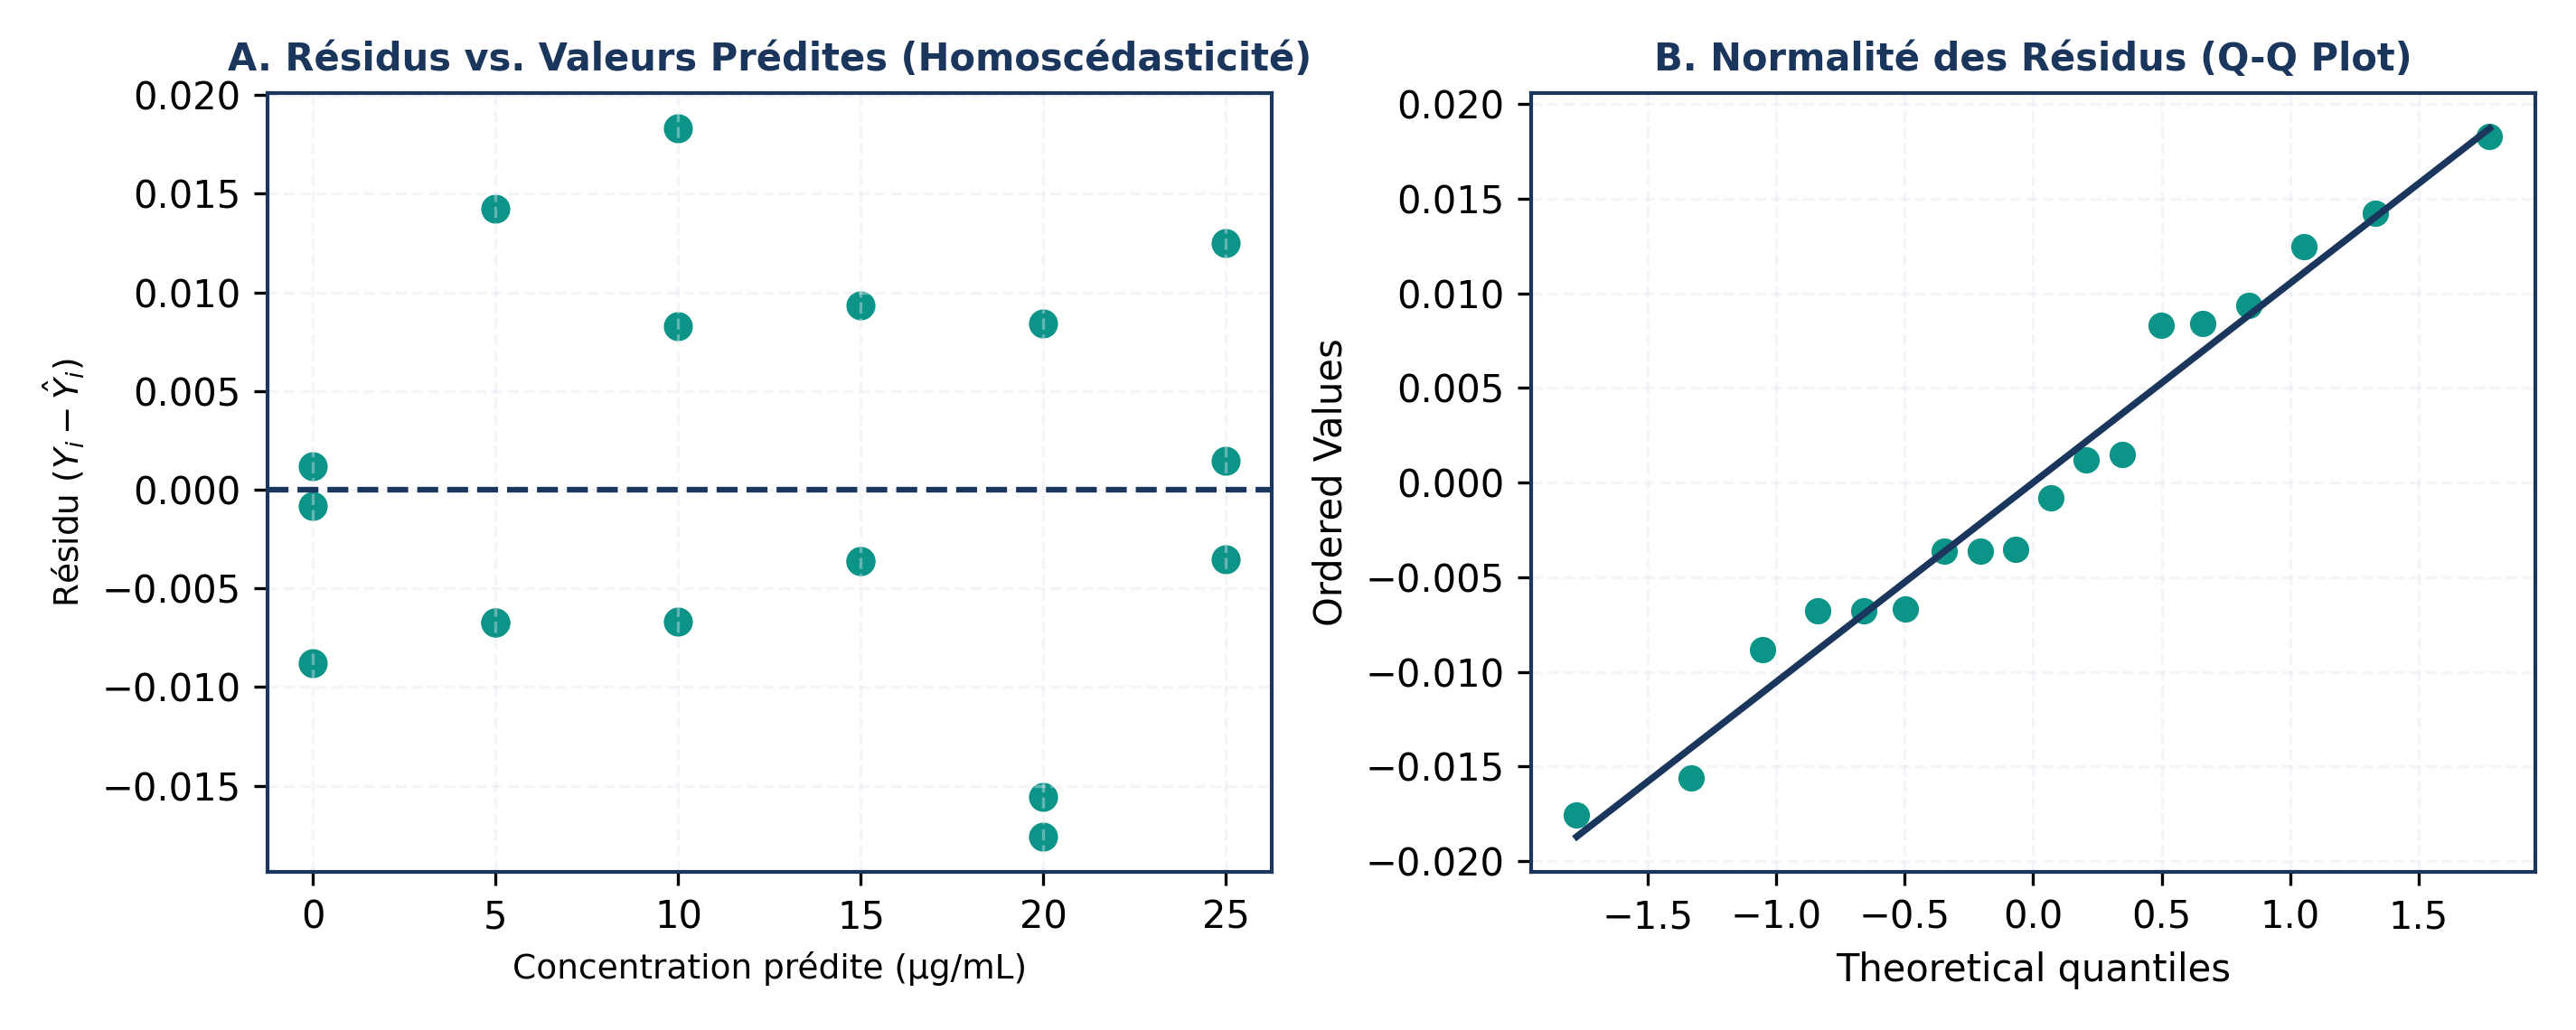
\includegraphics[width=0.86\linewidth]{../../sources/figures/fig03_residuals_diagnostics.png}
\end{center}
\textbf{Guide d'interprétation visuelle pour le biologiste :}
\begin{itemize}[leftmargin=*, label=\faAngleRight]
  \item \textbf{Résidus vs Valeurs Ajustées (Haut Gauche) :} Vérifie la linéarité. Les résidus doivent s'éparpiller aléatoirement autour de la ligne horizontale $0$ sans former de profil en parabole ou en $U$ (qui trahirait une cinétique non linéaire).
  \item \textbf{Diagramme Quantile-Quantile Normal (Q-Q Plot, Haut Droit) :} Vérifie la normalité. Les résidus standardisés doivent s'aligner rigoureusement sur la droite diagonale en pointillés. Un décrochage aux extrémités signale des queues lourdes ou des points atypiques.
  \item \textbf{Graphique Scale-Location (Bas Gauche) :} Vérifie l'homoscédasticité en traçant $\sqrt{|\text{Résidus standardisés}|}$. Une ligne de tendance horizontale confirme que le bruit optique ne croît pas avec l'absorbance.
  \item \textbf{Résidus vs Levier \& Distance de Cook (Bas Droit) :} Identifie les points influents. Les points possédant un levier élevé ($h_{ii}$) et une forte distance de Cook ($D_i > 1$) agissent comme un bras de levier et faussent la pente de l'étalonnage.
\end{itemize}
\end{figurebox}

\section{Limites Analytiques Réglementaires (ICH Q2R1 : LOD \& LOQ)}

D'après les normes internationales de validation bioanalytique (ICH Q2R1) :
\begin{equation*}
  \mathbf{LOD = \frac{3.3 \cdot s_{y/x}}{a}} \quad \text{(Limite de Détection)} \qquad\qquad \mathbf{LOQ = \frac{10 \cdot s_{y/x}}{a}} \quad \text{(Limite de Quantification)}
\end{equation*}

\begin{biobox}{Différence Biologique Cruciale entre LOD et LOQ}
\begin{itemize}[leftmargin=*, label=\faAngleRight]
  \item \textbf{LOD :} Plus faible concentration d'analyte qui produit un signal discernable avec certitude du bruit de fond du blanc ($S/N \ge 3.3$). \textit{À cette concentration, on sait que la molécule est présente, mais on ne peut pas quantifier sa valeur exacte.}
  \item \textbf{LOQ :} Plus faible concentration qui peut être dosée avec une exactitude et une fidélité acceptables ($S/N \ge 10$, $RSD \le 15\%$). \textit{Toute concentration mesurée inférieure à la LOQ doit être rapportée dans le cahier de laboratoire comme « $<$ LOQ » et non comme une valeur numérique chiffrée.}
\end{itemize}
\end{biobox}

\section{Exercices d'Application \& Solutions}

\begin{exercicebox}{Exercice 1 : Étalonnage Bradford \& Validation Analytique}
Un biochimiste prépare une gamme étalon d'albumine bovine (BSA) à $n = 5$ concentrations pour étalonner un spectrophotomètre à $595\,\text{nm}$ :
\begin{center}
\small
\begin{tabular}{lccccc}
\toprule
\textbf{Tube} & 1 & 2 & 3 & 4 & 5 \\
\midrule
\textbf{Concentration BSA ($x_i$, $\mu\text{g/mL}$)} & 2.0 & 4.0 & 6.0 & 8.0 & 10.0 \\
\textbf{Absorbance $A_{595}$ ($y_i$)} & 0.125 & 0.245 & 0.380 & 0.495 & 0.635 \\
\bottomrule
\end{tabular}
\end{center}
\textbf{Données calculées :} $\sum x_i = 30.0$, $\sum y_i = 1.880$, $\sum x_i^2 = 220.0$, $\sum y_i^2 = 0.868775$, $\sum x_i y_i = 13.820$.
\begin{enumerate}[label=\textbf{\alph*.}]
  \item Calculez $SS_{xx}$, $SS_{yy}$ et $SP_{xy}$.
  \item Déterminez le coefficient de corrélation linéaire de Pearson ($r$).
  \item Calculez la pente $a$, l'ordonnée à l'origine $b$ et écrivez l'équation de la droite d'étalonnage.
  \item Calculez le coefficient de détermination $R^2$. La méthode satisfait-elle le critère de validation accréditée ($R^2 \ge 0.995$) ?
  \item Calculez les résidus $e_i = y_i - \hat{y}_i$ pour les 5 tubes. Vérifiez numériquement la propriété fondamentale de régression $\sum e_i = 0$ et déduisez-en $s_{y/x}$.
\end{enumerate}
\end{exercicebox}

\begin{solutionbox}{Solution : Exercice 1}
\begin{enumerate}[label=\textbf{\alph*.}]
  \item \textbf{Calcul des sommes d'écarts :}
  \begin{align*}
    SS_{xx} &= \sum x_i^2 - \frac{(\sum x_i)^2}{n} = 220.0 - \frac{30.0^2}{5} = 220.0 - 180.0 = \mathbf{40.0} \\
    SS_{yy} &= \sum y_i^2 - \frac{(\sum y_i)^2}{n} = 0.868775 - \frac{1.880^2}{5} = 0.868775 - 0.706880 = \mathbf{0.161895} \\
    SP_{xy} &= \sum x_i y_i - \frac{(\sum x_i)(\sum y_i)}{n} = 13.820 - \frac{30.0 \times 1.880}{5} = 13.820 - 11.280 = \mathbf{2.540}
  \end{align*}
  \item \textbf{Coefficient de Pearson ($r$) :}
  \begin{equation*}
    r = \frac{SP_{xy}}{\sqrt{SS_{xx} \cdot SS_{yy}}} = \frac{2.540}{\sqrt{40.0 \times 0.161895}} = \frac{2.540}{\sqrt{6.4758}} = \frac{2.540}{2.54476} = \mathbf{0.9981}
  \end{equation*}
  \item \textbf{Droite des moindres carrés :}
  \begin{align*}
    a &= \frac{SP_{xy}}{SS_{xx}} = \frac{2.540}{40.0} = \mathbf{0.0635\,\text{OD}/(\mu\text{g/mL})} \\
    b &= \bar{y} - a \bar{x} = \frac{1.880}{5} - 0.0635 \times \frac{30.0}{5} = 0.376 - 0.381 = \mathbf{-0.005\,\text{OD}}
  \end{align*}
  Équation : $\mathbf{\hat{y} = 0.0635\,x - 0.005}$.
  \item \textbf{Coefficient de détermination \& Décision :}
  \begin{equation*}
    R^2 = r^2 = (0.99813)^2 = \mathbf{0.9963} \quad (99.63\%)
  \end{equation*}
  Puisque $R^2 = 0.9963 \ge 0.995$, la gamme étalon satisfait rigoureusement le critère de linéarité internationale.
  \item \textbf{Calcul détaillé des résidus individuels ($e_i = y_i - \hat{y}_i$) :}
  \begin{itemize}[leftmargin=*, label=\faAngleRight]
    \item Tube 1 ($x_1=2.0$) : $\hat{y}_1 = 0.0635(2.0) - 0.005 = 0.1220 \implies e_1 = 0.125 - 0.1220 = \mathbf{+0.0030}$
    \item Tube 2 ($x_2=4.0$) : $\hat{y}_2 = 0.0635(4.0) - 0.005 = 0.2490 \implies e_2 = 0.245 - 0.2490 = \mathbf{-0.0040}$
    \item Tube 3 ($x_3=6.0$) : $\hat{y}_3 = 0.0635(6.0) - 0.005 = 0.3760 \implies e_3 = 0.380 - 0.3760 = \mathbf{+0.0040}$
    \item Tube 4 ($x_4=8.0$) : $\hat{y}_4 = 0.0635(8.0) - 0.005 = 0.5030 \implies e_4 = 0.495 - 0.5030 = \mathbf{-0.0080}$
    \item Tube 5 ($x_5=10.0$) : $\hat{y}_5 = 0.0635(10.0) - 0.005 = 0.6300 \implies e_5 = 0.635 - 0.6300 = \mathbf{+0.0050}$
  \end{itemize}
  \textbf{Somme des résidus :} $\sum e_i = +0.0030 - 0.0040 + 0.0040 - 0.0080 + 0.0050 = \mathbf{0.0000}$ !\\
  \textbf{Somme des carrés résiduelle ($SCR$) :}
  \begin{equation*}
    SCR = \sum e_i^2 = 10^{-6} \times (9 + 16 + 16 + 64 + 25) = 130 \times 10^{-6} = \mathbf{0.000130}
  \end{equation*}
  \textbf{Écart-type résiduel :} $s_{y/x} = \sqrt{\frac{SCR}{n - 2}} = \sqrt{\frac{0.000130}{3}} \approx \mathbf{0.00658\,\text{OD}}$.
\end{enumerate}
\end{solutionbox}

\begin{exercicebox}{Exercice 2 : Dosage d'un Extrait Hépatique Inconnu \& Limites LOD / LOQ}
À partir de la gamme étalon précédente ($a = 0.0635$, $b = -0.005$, $SS_{xx} = 40.0$, $\bar{x} = 6.0$, $\bar{y} = 0.376$, $s_{y/x} = 0.00894$) :
Un extrait d'homogénat hépatique de rat dilué au $1/100^{\text{e}}$ donne une absorbance moyenne de $y_0 = 0.376\,\text{OD}$ ($m = 1$).
La valeur critique de Student pour $df = 5 - 2 = 3$ est $t_{0.05}(3) = 3.182$.
\begin{enumerate}[label=\textbf{\alph*.}]
  \item Estimez la concentration $\hat{x}_0$ dans l'éprouvette diluée.
  \item Calculez l'erreur type $s_{\hat{x}_0}$ via la formule de Mandel et déterminez l'intervalle de confiance à 95\%.
  \item Calculez la concentration en protéines du tissu hépatique initial en g/L (facteur 100).
  \item Calculez la LOD et la LOQ de cette méthode analytique.
\end{enumerate}
\end{exercicebox}

\begin{solutionbox}{Solution : Exercice 2}
\begin{enumerate}[label=\textbf{\alph*.}]
  \item \textbf{Concentration estimée :}
  \begin{equation*}
    \hat{x}_0 = \frac{y_0 - b}{a} = \frac{0.376 - (-0.005)}{0.0635} = \frac{0.381}{0.0635} = \mathbf{6.00\,\mu\text{g/mL}}
  \end{equation*}
  \item \textbf{Erreur type de Mandel ($m = 1, y_0 = \bar{y}$) :}
  Comme $y_0 = \bar{y} = 0.376$, le terme d'éloignement $(y_0 - \bar{y})^2 = 0$ :
  \begin{align*}
    s_{\hat{x}_0} &= \frac{s_{y/x}}{a} \sqrt{1 + \frac{1}{n} + 0} = \frac{0.00894}{0.0635} \sqrt{1 + \frac{1}{5}} = 0.1408 \times \sqrt{1.20} \\
    &= 0.1408 \times 1.0954 = \mathbf{0.154\,\mu\text{g/mL}} \\[1mm]
    IC_{95\%}(\hat{x}_0) &= 6.00 \pm (3.182 \times 0.154) = 6.00 \pm 0.49 = \mathbf{[5.51 \,;\, 6.49]\,\mu\text{g/mL}}
  \end{align*}
  \item \textbf{Concentration dans l'homogénat hépatique natif :}
  Avec le facteur de dilution $\times 100$ :
  \begin{equation*}
    C_{\text{foie}} = 6.00\,\mu\text{g/mL} \times 100 = 600\,\mu\text{g/mL} = \mathbf{0.60\,\text{g/L}} \quad (\pm 0.049\,\text{g/L})
  \end{equation*}
  \item \textbf{Limites analytiques réglementaires (LOD \& LOQ) :}
  \begin{align*}
    \mathbf{LOD} &= \frac{3.3 \times s_{y/x}}{a} = \frac{3.3 \times 0.00894}{0.0635} = \frac{0.0295}{0.0635} = \mathbf{0.465\,\mu\text{g/mL}} \\[1mm]
    \mathbf{LOQ} &= \frac{10 \times s_{y/x}}{a} = \frac{10 \times 0.00894}{0.0635} = \frac{0.0894}{0.0635} = \mathbf{1.408\,\mu\text{g/mL}}
  \end{align*}
\end{enumerate}
\end{solutionbox}

\section*{Formulaire Récapitulatif \& Bonnes Pratiques}
\begin{center}
\resizebox{\linewidth}{!}{%
\begin{tabular}{lll}
\toprule
\textbf{Paramètre Statistique} & \textbf{Formule Mathématique} & \textbf{Signification en Laboratoire} \\
\midrule
Pente de sensibilité ($a$) & $a = SP_{xy} / SS_{xx}$ & Signal optique généré par unité de concentration \\
Ordonnée à l'origine ($b$) & $b = \bar{y} - a\bar{x}$ & Signal d'absorbance du blanc réactionnel ($X = 0$) \\
Variance résiduelle ($s_{y/x}^2$) & $s_{y/x}^2 = \frac{\sum (y_i - \hat{y}_i)^2}{n - 2}$ & Bruit de fond instrumental aléatoire \\
Coefficient de détermination & $R^2 = 1 - (SCR / SCT)$ & Qualité globale de linéarité ($\ge 0.995$) \\
Incertitude inverse (Mandel) & $s_{\hat{x}_0} = \frac{s_{y/x}}{a} \sqrt{\frac{1}{m} + \frac{1}{n} + \frac{(y_0 - \bar{y})^2}{a^2 SS_{xx}}}$ & Précision réelle du dosage de l'échantillon \\
Limite de Détection (LOD) & $\text{LOD} = 3.3 \cdot s_{y/x} / a$ & Plus petite concentration discernable du bruit \\
Limite de Quantification (LOQ) & $\text{LOQ} = 10 \cdot s_{y/x} / a$ & Plus petite concentration dosable avec exactitude \\
\bottomrule
\end{tabular}%
}
\end{center}

\end{document}
